\documentclass[final]{beamer}

% ====================
% Packages
% ====================

\usepackage[T1]{fontenc}
\usepackage{lmodern}
\usepackage[size=custom,width=120,height=72,scale=1.0]{beamerposter}
\usetheme{gemini}
% \usecolortheme{uchicago}  % Stanford theme is already set
\usepackage{amsmath}
\usecolortheme{stanford}
\usepackage{graphicx}
\usepackage{booktabs}
\usepackage{tikz}
\usetikzlibrary{calc,arrows.meta,positioning}

\usepackage{pgfplots}
\pgfplotsset{compat=1.18}  % Use the latest compatible version (check your pgfplots manual)
\usepackage{tabularx} % For better table formatting
\usepackage{ragged2e} % For justified text in tables
\usepackage{changepage} % for adjustwidth environment
\usepackage{subcaption}
\usepackage{balance}

\usepackage{biblatex}
\bibliography{bibliography.bib}


% ====================
% Lengths
% ====================

% If you have N columns, choose \sepwidth and \colwidth such that
% (N+1)*\sepwidth + N*\colwidth = \paperwidth
\newlength{\sepwidth}
\newlength{\colwidth}
\setlength{\sepwidth}{0.025\paperwidth}
\setlength{\colwidth}{0.3\paperwidth}

\newcommand{\separatorcolumn}{\begin{column}{\sepwidth}\end{column}}


\title{Dynamic Quantization of LLMs via Reinforcement Learning (DynaQuant)}

\author{Oleg Roshka\inst{1}, Ilia Badanin\inst{2,*}}
\institute{\inst{1} Department of Computer Science, Stanford University \quad \inst{2} School of Computer and Communication Sciences, EPFL \quad \inst{*} Invited Collaborator}


% ====================
% Footer (optional)
% ====================

\footercontent{
	\href{https://github.com/olegroshka/rl-dynamic-quant}{github repo link} \hfill  % Replace with your repo
	CS 234 (2025 Winter) Final Project Poster Session \hfill
	\href{mailto:oros@stanford.edu}{oros@stanford.edu}, \href{mailto:ilia.badanin@epfl.ch}{ilia.badanin@epfl.ch}}  % Replace with your email
% (can be left out to remove footer)

% ====================
% Logo (optional)
% ====================

% use this to include logos on the left and/or right side of the header:
% \logoright{\includegraphics[height=7cm]{logos/cs-logo-maroon.png}}
% \logoleft{\includegraphics[height=7cm]{logos/cs-logo-maroon.png}}

% ====================
% Body
% ====================

\begin{document}
	
	% This adds the Logos on the top left and top right
	\addtobeamertemplate{headline}{}
	{
		\begin{tikzpicture}[remember picture,overlay]
			%   \node [anchor=north west, inner sep=3cm] at ([xshift=0.0cm,yshift=1.0cm]current page.north west)
			%   {\includegraphics[height=5.0cm]{stanford_logos/Stanford-CS.png}}; % uc-logo-white.eps
			\node [anchor=north east, inner sep=3cm] at ([xshift=0.0cm,yshift=2.5cm]current page.north east)
			{
\includegraphics[height=7.0cm]{stanford_logos/Block_S_2_color.png}};
		\end{tikzpicture}
	}
	
	\begin{frame}[t]
		\begin{columns}[t]
			\separatorcolumn
			
			\begin{column}{\colwidth}
				
				\begin{block}{Introduction}
					Large Language Models (LLMs) are powerful but resource-intensive. Quantization reduces model size and speeds up inference, but uniform quantization can be suboptimal. We propose a \textbf{dynamic}, per-layer quantization approach using Reinforcement Learning (RL) to find an optimal mixed-precision scheme during fine-tuning. This balances accuracy and memory footprint.
					
					\vspace{0.8em}
					\textbf{Key points:}
					\begin{itemize}
						\item \textbf{Motivation:} Exploit the fact that not all layers are equally sensitive to precision loss.
						\item \textbf{Approach:} Use \textbf{PPO} to pick layer-specific quantization types (e.g. nf4, fp4, int8, fp16), then do short fine-tuning to recover from possible performance drops.
						\item \textbf{Key Idea:} Adaptive fine-tuning after \textbf{each} layer's quantization captures the dynamic interaction between layers.
						\item \textbf{Goal:} Learn a per-layer quantization policy for LLMs that optimizes accuracy and memory usage.
					\end{itemize}
					
				\end{block}
				
				\begin{block}{Related Work}
					Our work builds upon several key areas:
					
					\begin{itemize}
						\item \textbf{LLM Quantization:} Techniques like GPTQ \cite{frantar2022gptq}, QLoRA \cite{dettmers2023qlora}, bitsandbytes \cite{dettmers2022llmint8} and extreme LLM compression efforts \cite{egiazarian2024extreme,malinovskii2024pvtuning} have demonstrated the effectiveness of quantization for LLMs.
						\item \textbf{RL for Architecture Search:} Methods like NASNet \cite{zoph2016neural} and APQ \cite{wang2020apq} use RL to optimize neural network architectures and quantization.
						\item \textbf{Mixed-Precision Quantization:} HAWQ \cite{dong2019hawq} and other methods explore layer-wise bit-width selection.
					\end{itemize}
					
					Our approach differs by using RL to \emph{dynamically} determine the mixed quantization scheme \emph{during} fine-tuning, allowing the model to adapt to the specific quantization choices.
					
				\end{block}
				
				\begin{block}{Reinforcement Learning Environment}
					\begin{columns}[T]
						\begin{column}{0.6\linewidth}
							\begin{figure}[ht]
								\centering
								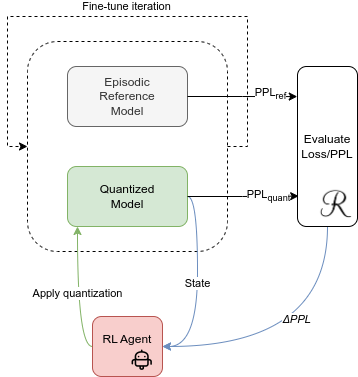
\includegraphics[width=\linewidth]{dynaq-scheme.png}
								\caption{RL-based dynamic quantization loop. Agent picks a quant type for the current layer, then fine-tunes and compares performance (losses/perplexities).}
							\end{figure}
						\end{column}
						\begin{column}{0.4\linewidth}
							\begin{itemize}
								\item \textbf{State:} Layer statistics (weight mean/std, gradient norm, attention entropy), current layer index, previous layer's quantization, and EMA of rewards.
								\item \textbf{Action:} Choice of quantization type: \{`nf4`, `fp4`, `int8`, `fp16`, `bf16`, `fp32`\}.
								\item \textbf{Reward:} Combination of perplexity difference (sigmoid-shaped), KL divergence, attention entropy difference, and memory savings.
								\item \textbf{Episode:} Quantizing all layers of the model sequentially.
								\item \textbf{Adaptive Fine-tuning:} Crucially, we fine-tune \emph{both} the quantized model \emph{and} an episodic reference model after \emph{each} layer's quantization, using \emph{identical} training data, for a fixed number of steps. This captures the dynamic impact of quantization.
							\end{itemize}
						\end{column}
					\end{columns}
				\end{block}
				
			\end{column}
			
			\separatorcolumn
			
			\begin{column}{\colwidth}
				
				\begin{block}{Reward Function (Multi-Objective)}
					We define the per-layer reward as a weighted sum of performance, distribution alignment, attention preservation, and memory savings:
					\[
					\begin{aligned}
						R \;=\; &w_{\mathrm{perf}}\; \sigma\!\bigl(\alpha\,(\mathrm{PPL}_{\mathrm{ref}} - \mathrm{PPL}_{\mathrm{quant}})\bigr) \\
						&\quad -\; w_{\mathrm{KL}}\;\mathrm{KL}\bigl(p_{\mathrm{quant}}\|\;p_{\mathrm{ref}}\bigr) \\
						&\quad +\; w_{\mathrm{entropy}}\,\bigl(\mathrm{Ent}_{\mathrm{quant}} - \mathrm{Ent}_{\mathrm{ref}}\bigr) \\
						&\quad +\; w_{\mathrm{memory}}\;\mathrm{MemSave}.
					\end{aligned}
					\]
					\textbf{Interpretation:}
					\begin{itemize}
						\item \(\mathrm{PPL}_{\mathrm{ref}} - \mathrm{PPL}_{\mathrm{quant}}\): difference in perplexities, run through a sigmoid (\(\sigma\)) to keep reward in (0,1).
						\item \(\mathrm{KL}(p_{\mathrm{quant}}\|\,p_{\mathrm{ref}})\): penalize large distribution shift.
						\item \(\mathrm{Ent}_{\mathrm{quant}} - \mathrm{Ent}_{\mathrm{ref}}\): preserve attention diversity.
						\item \(\mathrm{MemSave}\): bit savings relative to a 16-bit baseline, scaled by fraction of total params in that layer.
					\end{itemize}
					\vspace{0.2em}
					We also employ an exponential moving average (EMA) of the total reward to stabilize training updates in PPO.
				\end{block}
								
				\begin{block}{Implementation}
					\begin{itemize}
						\item \textbf{Model:} GPT-2 (small, medium, large).
						\item \textbf{Quantization:} `bitsandbytes` library and custom.
						\item \textbf{RL Algorithm:} Proximal Policy Optimization (PPO).
						\item \textbf{Fine-tuning Data:} CommonsenseQA.
						\item \textbf{Evaluation:} Perplexity, memory usage and inference speed. Datasets: BoolQ, PIQA
						\item \textbf{Infrastructure:} Training performed on H100 GPUs using the Modal platform. We gratefully acknowledge Modal for providing a free compute budget.
					\end{itemize}
				\end{block}
				
				\begin{block}{Results}
					\begin{table}[h!]
						\centering
						\caption{Results on GPT-2 Small (PIQA).  We compare perplexity (PPL), accuracy (Acc), and peak GPU memory (Mem).  All deltas (\%) are computed relative to FP32 as the baseline.}
						\resizebox{\linewidth}{!}{%
							\begin{tabular}{lrrrrrr}
								\toprule
								\textbf{Method} & \textbf{PPL} & \boldmath$\Delta$\textbf{PPL(\%)} & \textbf{Acc(\%)} & \boldmath$\Delta$\textbf{Acc(pp)} & \textbf{Mem (MB)} & \boldmath$\Delta$\textbf{Mem(\%)} \\
								\midrule
								Baseline (FP32) & 25.31 & ---    & 60.72 & ---   & 574.22 & ---    \\
								Baseline (FP16) & 25.31 & +0.01\% & 60.72 & +0.00 & 422.69 & -26.38\% \\
								Uniform NF4     & 22.66 & -10.47\% & 60.77 & +0.05 & 300.95 & -47.60\% \\
								DynaQuant (mixed)& 21.44 & -15.29\% & 61.53 & +0.82 & 464.29 & -19.14\% \\
								\bottomrule
							\end{tabular}
						} % end resizebox
						\vspace{0.4em}
						\footnotesize
						\justifying
						\textbf{Notes:} 
						The reported DynaQuant configuration uses a mixed schema 
						\{\texttt{fp16, int8, fp16, nf4, fp16, int8, fp16, int8, fp4, nf4, int8, fp4}\}.
						Perplexities are scaled by dividing raw values by 100. For instance, a raw PPL of 2531.21 is shown as 25.31.
						FP32 is the reference baseline. FP16 yields a memory reduction of about 26\% with negligible changes in perplexity and accuracy.
						Uniform NF4 offers a larger perplexity drop (-10.47\%) while cutting memory nearly in half.
						\textbf{DynaQuant} achieves the best overall trade-off: a -15.29\% drop in perplexity, a +0.82 percentage point gain in accuracy, and a -19.14\% memory reduction relative to FP32.
						\label{tab:results}
					\end{table}
				\end{block}
				
				
				\begin{block}{Training Dynamics}
					\vspace{-0.6em}
					\begin{figure}[ht]
						\centering
						\begin{subfigure}[b]{0.3\linewidth}
							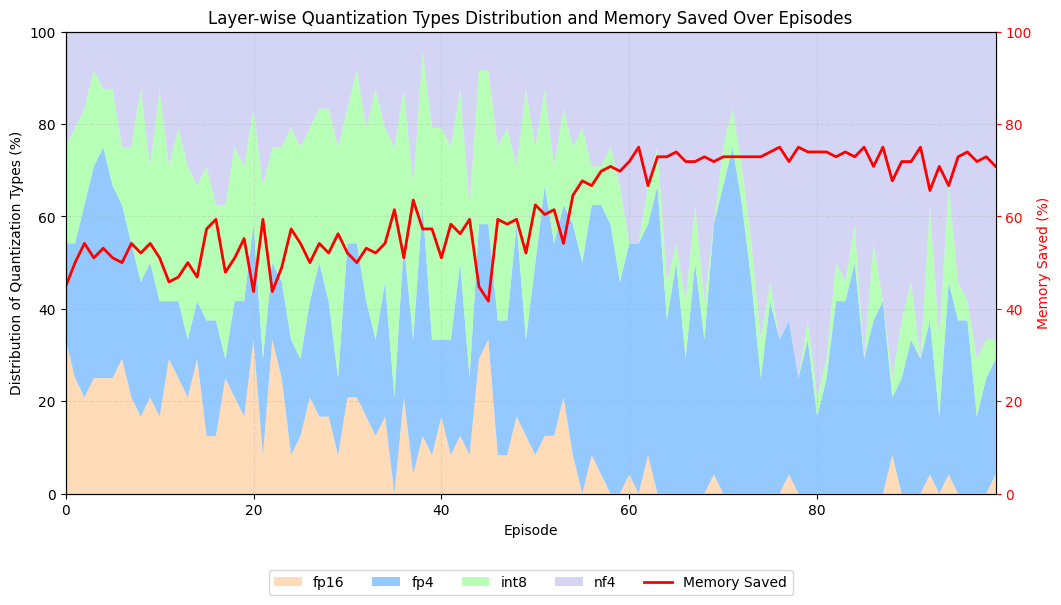
\includegraphics[width=\linewidth]{layer_quantization_plot.png}
							\caption{\small Quantization types distribution and memory savings over episodes.}
						\end{subfigure}
						\hfill
						\begin{subfigure}[b]{0.32\linewidth}
							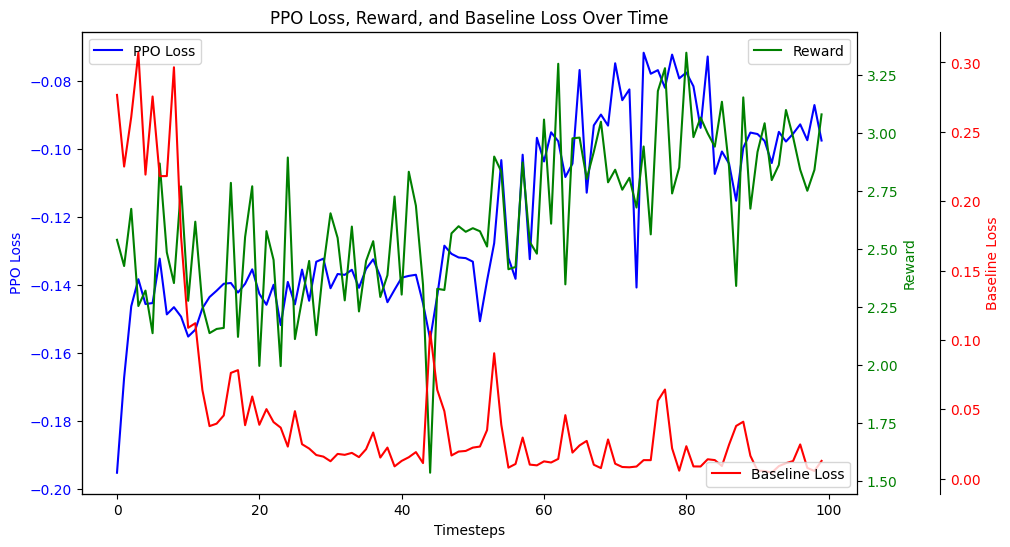
\includegraphics[width=\linewidth]{losses_plot.png}
							\caption{\small Training metrics over episodes: reward, PPO loss, and baseline loss.}
						\end{subfigure}
						\hfill
						\begin{subfigure}[b]{0.27\linewidth}
							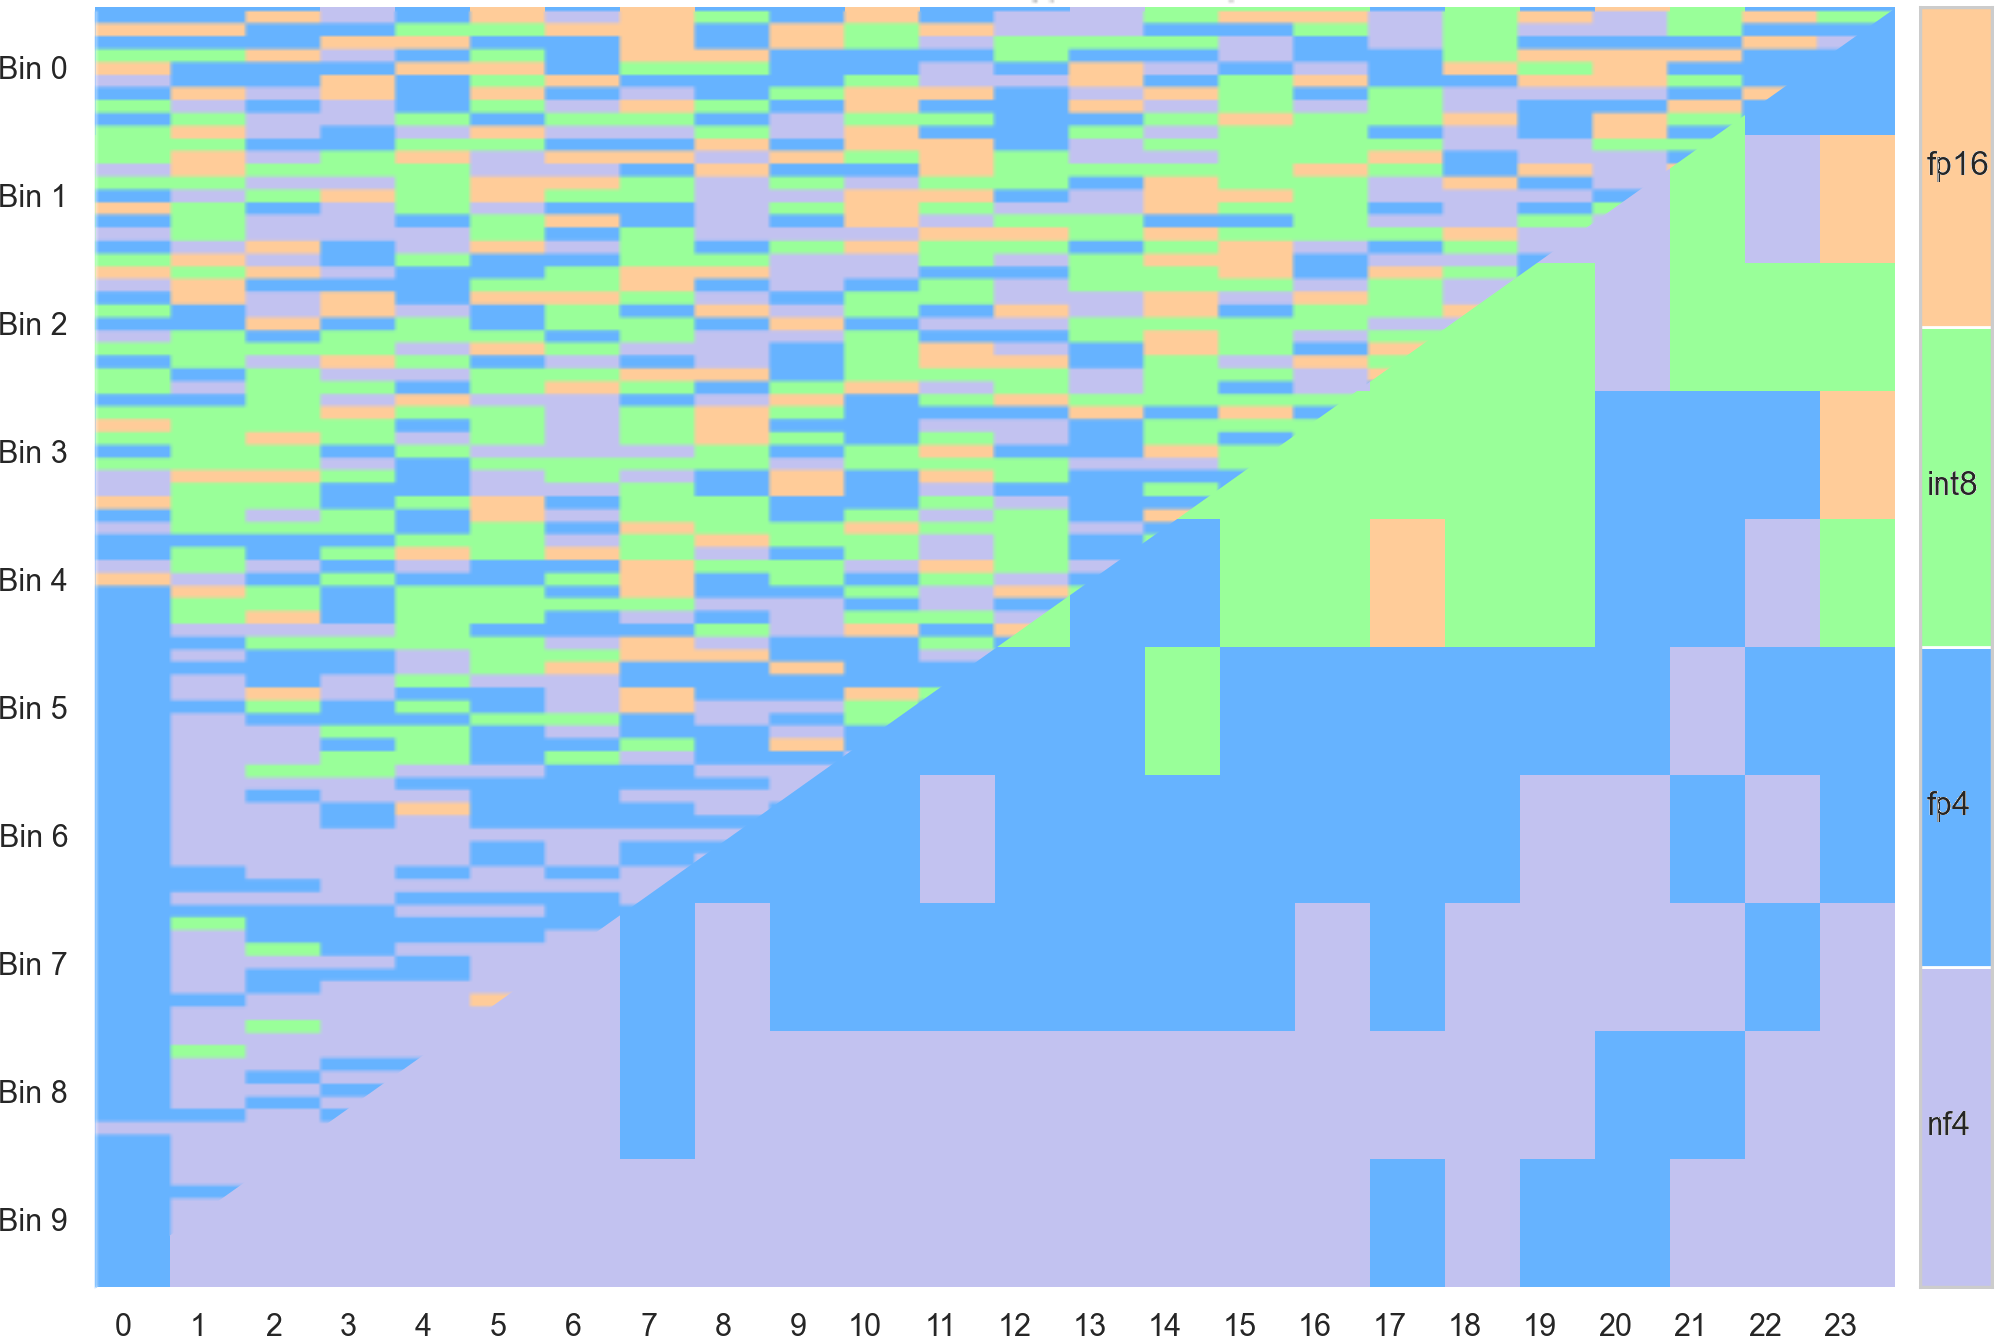
\includegraphics[width=\linewidth]{binnobin.png}
							\caption{\small Binned quantization of layers across 100 episodes}
							\label{subfig:reward_trend}
						\end{subfigure}
						
						\caption{\small The evolution of quantization types over episodes in the training phase, the plots show the trade-off between memory savings and PPO loss - as memory savings increase, the PPO loss tends to increase as well, but the reward overall increases.}
						\label{fig:training_plots}
					\end{figure}					
				\end{block}
				
			\end{column}
			
			\separatorcolumn
			
			\begin{column}{\colwidth}
				
				\begin{block}{Observations}
					\begin{itemize}
						\item \textbf{Reward Dynamics:} Although the reward trends upward as the agent refines its per-layer decisions, it can be noisy. Sudden drops or oscillations may occur, especially when reward weights, batch sizes, or the number of fine-tuning steps change.
						\item \textbf{Policy Sensitivity:} By adjusting reward weights, one can steer the agent toward more aggressive compression (prioritizing memory savings) or more performance-preserving (accuracy-focused) quantization strategies.
						\item \textbf{Validation Loss Stability:} Even with layer-by-layer quantization, the quantized model's validation loss stays reasonably close to that of the reference, thanks to short post-quantization fine-tuning.
						\item \textbf{Layer-Specific Choices:} Some layers often tolerate lower-precision (e.g.\ 4-bit), while more sensitive layers might require int8 or float16.
						\item \textbf{Compute Cost vs.\ Benefits:} This approach is compute-intensive. However, it can be justified by the overall memory/accuracy trade-off gains in scenarios where quality on user specific data sets is paramount.
					\end{itemize}
				\end{block}
				
				
				
				\begin{block}{Conclusion and Future/In-progress Work}
					We presented an RL-based approach for dynamic, per-layer quantization of LLMs.  Our method learns a policy that balances accuracy (perplexity) and memory usage, achieving a better trade-off than uniform quantization.  Key features include:
					
					\begin{itemize}
						\item \textbf{Dynamic:}  The policy adapts to each layer's characteristics.
						\item \textbf{Adaptive Fine-tuning:} Captures the interplay between quantized layers.
						\item \textbf{Multi-Objective Reward:}  Balances perplexity, KL divergence, entropy, and memory.
					\end{itemize}
					
					Future work includes:
					\begin{itemize}
						\item Scaling to larger models (e.g., \texttt{DeepSeek-R1-Distill-Qwen-1.5B} or \texttt{phi-2}).
						\item Hyperparameter tuning and exploration of different reward weightings.
						\item Adding a "skip" action to the policy, allowing it to choose not to quantize a layer.
						\item Exploring a policy network with a transformer architecture to leverage past decisions for better future choices. With enough training on diverse models/datasets, such a policy could infer a robust mixed-precision scheme from only a few fine-tuning steps for new scenarios.
					\end{itemize}
				\end{block}
				
				\begin{block}{References}
					\balance					
					\printbibliography
				\end{block}
				
			\end{column}
			
			\separatorcolumn
		\end{columns}
	\end{frame}
	
\end{document}